\section{\sysname~Design}
\label{sec:design}

% Design goals:
%   A research control plane
%     Easy to use, adjust source code, modification points
%     Full system stack: controller (load balancer), worker(s), load generation, containers, workloads, simulation
%     Configurable, lots of knobs to adjust things easily
%     Tracking of metrics/resources/system events
%   low-variance! and low(ish)-overhead control plane
%   No frivilous features, not too complicated

\sysname's design is guided by our experience of OpenWhisk performance, and by our goals of providing predictable performance, modularity, and a control plane for reliable FaaS research.

% \vspace*{-8pt}
\subsection{Architecture and Overview}
\label{sec:design:arch}

The \sysname~control plane is spread out across a load balancer and the individual workers, and sits above the containerization layers. 
We intend for \sysname~to be the narrow waist~\cite{popa_http_2010} in the FaaS ecosystem: with optimizations for DAG scheduling~\cite{zhou_qos-aware_2022}, state handling~\cite{sreekanti2020cloudburst}, and horizontal scaling~\cite{faaslb-hpdc22} implemented above it, and sandboxing and containerization below it.  
This architecture was motivated by the key question: \emph{Can fast FaaS control planes be implemented with strict layering and separation of concerns?}


We have found that most of the control plane overhead is in the workers, and hence optimizing the worker performance is our major focus.
%
Our architecture is \textbf{worker-centric}, and places more performance and load-management responsibility on the individual workers, instead of a more ``top-down'' centralized approach favored by prior work such as Atoll~\cite{singhvi2021atoll} and others~\cite{kaffes_centralized_2019, kaffes_hermod_2022}.
Top-down resource management requires a consistent global view of the cluster, and is complementary to our work. 
Predictive techniques for load-balancing, prefetching, scheduling, function-sizing can all be effective, but we want to explore the performance characteristics and limits of \emph{reactive} control planes that work with unmodified container runtimes. 

\begin{figure}
  \centering 
  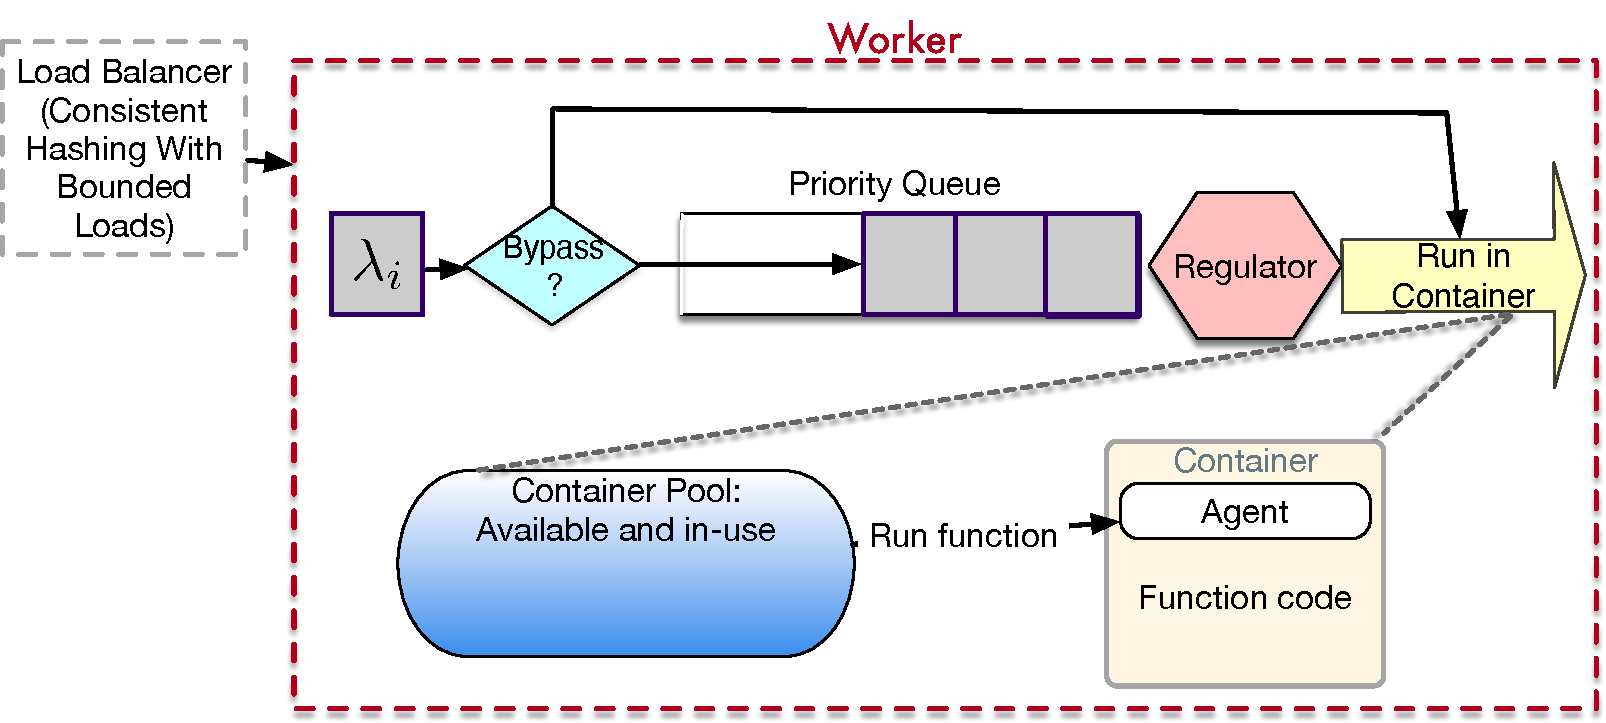
\includegraphics[width=0.6\textwidth]{iluvatar/figs/il76-q.pdf}
    % \vspace*{-6pt}
  \caption{\sysname~has a worker-centric architecture. A per-worker queue helps schedule functions, and regulate load and overcommitment. }
  \label{fig:arch}
  % \vspace*{-6pt}
\end{figure}

\sysname's main components are shown in Figure~\ref{fig:arch}.
Clients/users invoke functions using an HTTP or RPC API, with the main operations being \texttt{register, invoke, async\_invoke, and prewarm}.
Workers also provide load and status information to the load-balancer. 
We use stateless load-balancing, by using variants of consistent hashing with bounded loads (CH-BL), which have been proposed for FaaS recently~\cite{faaslb-hpdc22}. 
This is a locality-aware scheme, which runs functions on the same servers to maximize warm starts, and forwards them to other servers only when the server's load exceeds some pre-specified load-bound.


Continuing on the worker-centric theme, the worker API is a subset and almost completely identical to the overall API, and functions can be launched directly on a worker for single-worker setups and benchmarking, without going through a load-balancer and adding unnecessary latency.
The workers implement various latency-hiding and burst-mitigation techniques. 
All functions are launched inside containers, and dealing with the container layer is a major part of the worker. 
Each worker maintains a container pool of initialized containers for facilitating warm starts, and has an invocation queue for handling dynamic loads.
Function characteristics such as their cold and warm execution times are captured in various data-structures and are made available using APIs for developing data-driven resource management policies.

An important contribution and component of \sysname~is its principled support for function overcommitment based on its queuing architecture.
In many environments, like public FaaS providers, function resources cannot be overcommitted. 
However, the actual function resource usage is often significantly less compared to their requested \quotes{size}.
This difference is the motivation behind recent \quotes{right sizing} work~\cite{akhtar_cose_2020, guo_decomposing_2022, tian_owl_2022, eismann2021sizeless, kotni2021faastlane}, and can significantly improve system utilization.
Through its queue-based architecture, \sysname~supports a wide range of overcommitment scenarios, including no overcommitment, which is absent from OpenWhisk.
By default, OpenWhisk does not overcommit memory, but can  overcommit CPUs, which introduces performance interference and potential SLA violations for functions. 



%%%%%%%%%%%%%%%%%%%%%%%%%%%%%%%%%%%%%%%%


% \subsection{Function handling in the workers}
% \vspace*{-8pt}
\subsection{Function Lifecycle}
\label{sec:design:lifecycle}

%Function lifecycle is controlled by three main \sysname~worker API calls.
New functions first must be \emph{registered}, which entails downloading and preparing its container disk image.
The container images are fetched from DockerHub or some other image repository.
Container images are composed of multiple copy-on-write layers, and we prepare the images by selecting the relevant layers for the operating system and CPU architecture.
The images consist of the user-provided function code and our agent, which is a simple Python HTTP server that runs in each container. 
%How functions are registered and prepared to run by the control plane isn't immediately interesting research-wise, so we choose to do these out-of-band.
%
Registered functions can then be directly \emph{invoked}, which triggers launching of the function's container.
The first invocation is usually a cold-start, which entails launching the container image from disk, or from a previous snapshot~\cite{ustiugov2021benchmarking, ao2022faasnap} if available. 
Each function container starts the agent which listens for and controls the actual function code execution. 
The agent has two simple commands, a \texttt{GET /} endpoint for simple status checking, and a \texttt{POST /invoke} to run an invocation with some arguments.
When the container is ready, the worker sends an HTTP request to the agent to start the function code execution. 
We detect the container's readiness using an inotify callback, which is a faster and more generic mechanism for notification compared to Docker's built-in API. 
%
Finally, when the function finishes execution, the HTTP call to the container's agent returns, and the container is marked as \quotes{available} in the container pool, to be potentially used for future invocations of the same function.

\begin{comment}
In the spirit of a fast \quotes{baseline} control plane and for isolation, \sysname~does not share containers across functions.
This is in contrast to SAND's application sandboxing~\cite{akkus_sand_2018}, SOCK's Zygote containers~\cite{oakes_sock_2018}, Nightcore~\cite{jia2021nightcore}, and even OpenFaaS~\cite{openfaas}.
%For example, recently proposed optimizations such as SAND's application sandboxing~\cite{akkus_sand_2018}, or SOCK's Zygote containers~\cite{oakes_sock_2018} share containers for concurrently running functions. 
% allow for functions to share a language runtime inside a container, or the same function to reuse 
% SAND's application sandboxing~\cite{akkus_sand_2018}, or SOCK's Zygote containers~\cite{oakes_sock_2018}. 
%We don't allow concurrent invocations of the same function to run in the same container like OpenFaaS~\cite{openfaas} or nightcore~\cite{jia2021nightcore}.
Our isolation model is similar to the public cloud providers. 
\end{comment}

Additionally, \sysname~introduces a standard \texttt{prewarm}  API call, which starts the function's container and the agent inside of it, and adds it to the container pool.
This reduces most of the cold-start overhead associated with the container.
Prewarming can both avoid a \quotes{thundering herd} of cold starts on worker startup, and be an optimization in which the control plane anticipates invocations and prepares containers for them. 
This allows for a systematic mechanism to implement various recently proposed predictive prewarm policies~\cite{roy2022icebreaker, shahrad_serverless_2020, silva_prebaking_2020}. 

%When a container is created, our agent is started up inside it.




\begin{figure}
\centering 
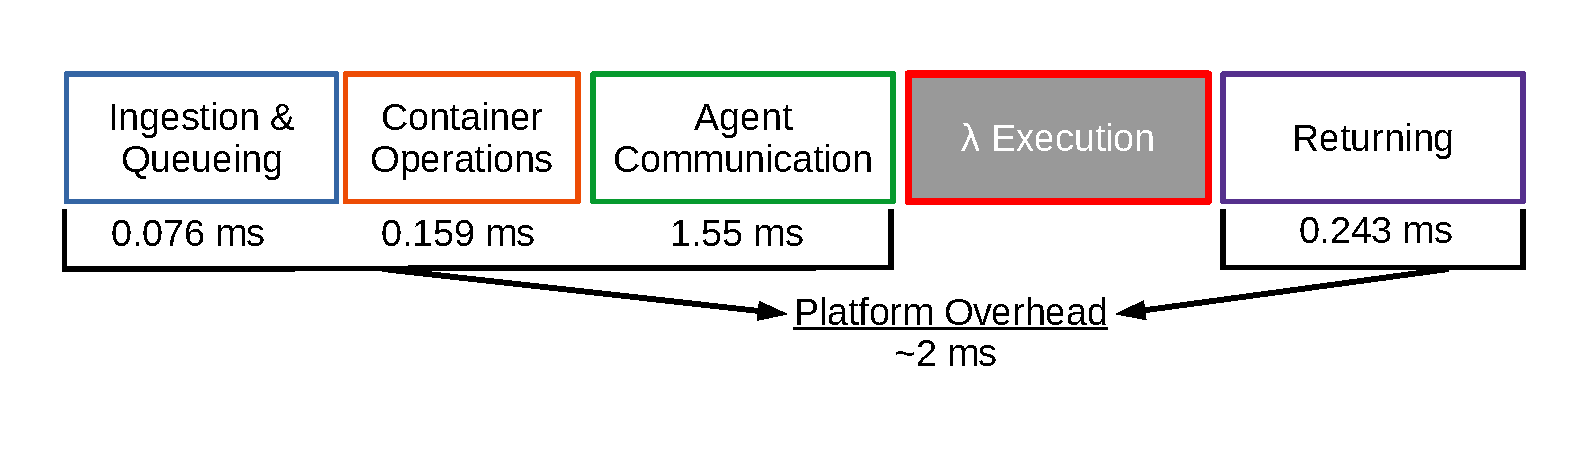
\includegraphics[width=0.6\textwidth]{iluvatar/figs/OverheadTimeline.pdf}
% \vspace*{-12pt}
\caption{The main components of the \sysname~overheads.}
\label{fig:timeline-flow}
  % \vspace*{\myfigspace}
  % \vspace*{-12pt}
\end{figure}


\noindent \textbf{Function Latency Breakdown.}
Throughout \sysname~and this paper, we are interested in three main performance metrics. 
The first is the end-to-end latency of function execution, also called the \emph{flow time}, shown in Figure~\ref{fig:timeline-flow}.
This in turn has two main components: the control plane overhead is the latency of \sysname~operations, which are mainly before the start of function execution.
The second component is the function execution time, which is determined by the function code, and the load on the system.
The function execution time is our baseline, and we compute the \emph{normalized} end-to-end latency by dividing the full latency by the execution time (also called the \emph{stretch}). 

A more detailed latency breakdown is shown in Table~\ref{tab:overheads}.
The majority of overhead comes from the communication with the agent which is over HTTP. 
This is a deliberate choice, since we wanted to be compatible with existing OpenWhisk function images.
This can be reduced by using faster IPC mechanisms like in Nightcore~\cite{jia2021nightcore}. 
However, these faster communication approaches would reduce compatibility, especially with functions deployed inside VMs.

For OpenWhisk, a similar latency breakdown shows that a large amount of time is spent reading/writing to CouchDB (up to half a second), and the rest of the slowdown occurs in the Invoker (OpenWhisk's worker) and is primarily due to its design and implementation. 
Interestingly, the load-balancer/controller for OpenWhisk adds less than 3ms of latency even under heavy load, indicating that the worker-level performance is relatively more important. 
This further motivates our worker-centric design and evaluation focus. 


\begin{table}
  \centering 
  \begin{tabular}{|c|c|r|}
    \hline
    Group & Function Name & Time (ms) \\
    \hline
    Ingestion \& Queuing & \begin{tabular}{@{}c@{}}invoke \\ sync\_invoke \\ enqueue\_invocation \\ add\_item\_to\_q \end{tabular} & \begin{tabular}{@{}c@{}}0.026 \\ 0.013 \\ 0.017 \\ 0.02 \end{tabular} \\
    \hline
    Container Operations & \begin{tabular}{@{}c@{}}spawn\_worker \\ dequeue \\ acquire\_container \\ try\_lock\_container \\ \end{tabular} & \begin{tabular}{@{}c@{}}0.029 \\ 0.02 \\ 0.096 \\ 0.014 \\ \end{tabular} \\
    \hline
    Agent Communication & \begin{tabular}{@{}c@{}}prepare\_invoke \\ call\_container \\ download\_result \\ \end{tabular} & \begin{tabular}{@{}c@{}}0.154 \\ 1.364 \\ 0.032 \\ \end{tabular} \\
    \hline
    Returning & \begin{tabular}{@{}c@{}}return\_container \\ return\_results \\ \end{tabular} & \begin{tabular}{@{}c@{}}0.017 \\ 0.266 \\ \end{tabular} \\
    \hline
  \end{tabular}
  \caption{Latency of different \sysname~worker components for a single warm invocation.}
    \label{tab:overheads}
\end{table}

%As we can see, the overheads are minimal. Some queuing, some agent communication, which totals to about 3ms. 
% \vspace*{-8pt}
\subsection{Worker Performance Optimizations}
\label{sec:design:worker}

To achieve this low latency function execution for heterogeneous and bursty workloads, \sysname~uses two key underlying design principles: resource caching, and asynchronous handling of function life-cycle events.

\subsubsection{Resource Caching}

The cornerstone design goal of \sysname~is to reduce jitter, which we accomplish by removing expensive operations from the function's critical path. 
Instead, we cache and reuse as many function resources as possible, which minimizes the \quotes{hot path} function invocation latency significantly.
This principle is applied in various worker components, which we describe below.
A fast \textbf{Container Pool Keep-alive} and cached \textbf{HTTP Clients} allow for efficient warm start invocations.
Pre-allocating and caching \textbf{Network Namespaces} shortens cold starts---a technique first used for rapid container provisioning~\cite{oakes_sock_2018};

\noindent \textbf{Container Keep-alive.}
The primary and exemplary application of resource caching is in the container keep-alive cache that \sysname~workers maintain.
The containers become \quotes{warm} when their function has finished execution, and become \quotes{available} for the next invocation of the same function. 
We maintain a pool of all in-use and available containers for each registered function.
This container cache implements classic eviction policies such as Least Recently Used (LRU), and size-aware policies like Greedy-Dual-Size-Frequency, as proposed in FaasCache~\cite{faascache-asplos21}. 

\noindent \textbf{Network Namespace Caching.}
For isolation, each container is provided with a virtual network interface and a network namespace.
Through performance profiling, we've found that creating this network namespace can add significant latency to container cold starts---as much as 100ms.
This is due to contention on a single global lock shared across all network namespaces~\cite{oakes_sock_2018}. 
To minimze this overhead, we maintain a pool of pre-created network namespaces that are assigned during container creation. 
The isolation is still maintained, since concurrently running containers do not share the namespace. 
%Avoiding this expensive operation on the critical path.

\noindent \textbf{HTTP Clients.}
The worker threads communicate with the in-container agent for launching the function code.
Instead of creating a new HTTP client for every invocation, we cache a client per container and use connection pooling. 
This affects all invocations (even warm starts), and reduces the control-plane overhead latency by up to $3ms$. 

\subsubsection{Async Function Life-Cycle Handling}

The second key design principle is to handle various aspects of the function's lifecycle asynchronously off the critical path.
\sysname~achieves this through background worker threads for certain tasks, and through its Rust implementation which heavily uses asynchronous functions, futures, and callbacks wherever possible. 

\noindent \textbf{Keep-alive eviction.}
One such aspect is maintaining the function keep-alive cache, and ensuring that new functions have enough free memory to launch without waiting on existing containers to be evicted first.
Traditionally, eviction decisions would be made in an online fashion, but picking victims and waiting for their removal creates high variance in function execution times. 
\sysname~performs container eviction from the keep-alive pool  periodically in the background, off the critical path. 
This is similar to the Linux kernel page-cache implementation. 
We maintain a minimum free-memory buffer for dealing with invocation bursts, and periodically sort the containers list for eviction based on caching policies from~\cite{faascache-asplos21}. 

\noindent \textbf{Function Queuing.}
An important component of \sysname's architecture is a per-worker function queue.
New invocations are first put into the queue, and are dispatched to the container backend by a queue monitoring thread. 
%only when sufficient resources are available.
This allows us to tolerate bursts of invocations, and regulate the server load. 
% Details of our queuing policies are presented in Section~\ref{sec:q}.

%%%%%%%%%%%%%%%%%%%%%%%%%%%%%%
% \vspace*{-8pt}
\subsection{Container Handling}
\label{sec:design:ctr}

\sysname~uses standard Linux containers for isolating and sandboxing function execution---a \quotes{vanilla} and conventional approach.  
Several exciting new isolation mechanisms for cloud functions
have been proposed: such as lightweight VMs~\cite{firecracker-nsdi20}, unikernels, WASM~\cite{shillaker2020faasm} and other language runtimes~\cite{graalvm}, etc. 
Importantly, the sandboxing affects the \emph{cold start} overheads, which account for a tiny fraction of all invocations (usually less than 1\%).
Our control plane design and performance optimizations are independent of the sandboxing mechanism, and we address the orthogonal problem of optimizing the \emph{warm starts}. 

The basic container operations we use are: i) Create a container/sandbox with specified resource limits and disk image/snapshot, ii) launch a task inside it for the agent, and iii) destroy the container.
Each container is launched with the CPU and memory resource limits. CPU limits are enforced with cgroup quotas. 
This limited API allows \sysname~to support \emph{multiple} container backends.


By default, we use containerd~\cite{containerd}, which is popular container library, also used by Docker. 
The very rich containerization ecosystem presents a large number of options, and examining their tradeoffs was a major part of \sysname's design process.
Importantly, the choice of containerization library impacts the cold-start times, and some library operations can take considerable time (100s of ms). 
High-level container frameworks like Docker are feature-rich and easy to use, but are typically used for long-running containers and are not optimized for latency.
Docker uses containerd under the hood, and it provides  more fine-grained control and slightly better latency.
Functions require a minimal containerization, and a lot of feature-complexity in these large containerization libraries can add to latency.
For instance, the crun~\cite{crun} library which is written in C takes about 150ms to launch a container, whereas containerd (written in Go) needs 300ms, and Docker needs 400ms. 

Using containerd allows us to use the OCI container specification~\cite{oci}, and makes it easier to support other container runtimes.
For instance, we also support the Docker container backend, which required only a minimal programming effort.
Containerd operates as a separate service, and we use it's RPC-based API, which contributes to some latency as well.
We contemplated writing our own optimized container runtime in Rust to avoid the overheads due to inter-process communication, extra process forks and system calls, and implement other cgroups and namespace optimizations. 
However, we ended up going with containerd to keep our control plane small and reusable across container runtimes.
We also wanted to investigate and tackle the challenge of getting predictable performance out of higher level containerization services that are not part of the same address space. 


\noindent \textbf{Simulation Backend.}
In addition to containerd and Docker containers, we also support a \quotes{null} container backend which is useful for simulations and evaluating control plane scalability.
%
Because of the scale and variety of FaaS workloads, using discrete event simulators for developing and evaluating resource management policies is often necessary.
%
For instance, the recent work on FaaS load balancing~\cite{faaslb-hpdc22} uses such a simulator for evaluating their policies at scale for different subsets of the Azure workload trace.
Usually, the simulation is used to augment and complement the \quotes{real} empirical evaluation of the same policies which are implemented in FaaS frameworks like OpenWhisk. 

However, a major methodological and practical issue is that the policy implementations, workload generation, and analysis, all need to be duplicated across the simulator and the real system.
This can lead to subtle and large divergences between the simulation and real environment. 
Moreover, the simulator cannot capture all the real-world dynamics and jitter, and can suffer from poor fidelity.

In order to aid researchers, \sysname~takes a different approach to simulations, and provides \emph{in-situ} simulations. 
Our \quotes{null} container backend does not run any actual function code, but instead sleeps for the function's anticipated execution time.
The rest of the control plane operates exactly as with real containers, and we still handle all other aspects of the function's lifecycle.
%
This allows us to simulate large systems and workloads. 
For evaluating any particular policy, researchers can use the simulator null-backend to evaluate control-plane overheads, warm-starts, etc., without requiring a large cluster.
Each \sysname~worker can \quotes{simulate} 100s of cores, since the CPU resources are only being consumed by the control plane, and not for running actual functions.
Alternatively, a large cluster can be simulated with multiple simulated workers. 

With this approach, \emph{there is minimal difference} between the simulation and the real system. 
Thus an experiment can be run in-situ or in-silico, following identical code paths.
The main distinction is that API calls to containerd are replaced with internal dummy function calls, and function invocations are converted to sleep statements.  
All control plane operations, control-flow, logging, resource limits enforcement, etc., are exactly the same as with the \quotes{real} \sysname.
This also helps with mocking and testing new policies. 

%%%%%%%%%%%%%%%%%%%%%%%%%


%%% Local Variables:
%%% mode: latex
%%% TeX-master: "paper"
%%% End:
